\documentclass[10pt,twocolumn,letterpaper]{article}
\usepackage[pagenumbers]{cvpr}
\usepackage[T1]{fontenc}
\usepackage{graphicx}
\usepackage{amsmath,amssymb}
\usepackage{booktabs}
\usepackage{balance}
\usepackage[breaklinks,colorlinks,citecolor=blue,urlcolor=blue,linkcolor=blue]{hyperref}
\usepackage[capitalize]{cleveref}
\def\confName{NOWAI}
\def\confYear{2026}
\begin{document}
\title{Predicting Reasoning-Model Costs from Shared Prefill Activations}
\author{Anonymous authors}
\maketitle

\begin{abstract}
Reasoning-model routers must estimate generation cost before choosing a model, yet output lengths vary across queries. We estimate route-specific costs from the prefill activations of a frozen 4B encoder, sharing features with the success predictor. Linear cost readouts require no target-model computation before route selection. We evaluate deterministic routing curves and calibration-selected policies on 6,500 new MMLU-Pro and 1,000 new Omni-MATH problems. Against training-median costs, a 75\% calibration target on MMLU-Pro gives 31.1\% lower spending and 1.29 points higher fresh accuracy. A 65\% target on Omni gives 24.9\% lower spending with an uncertain accuracy difference. Other targets show accuracy--cost tradeoffs. Original-test comparisons with alternative estimators provide mixed evidence. The benefit depends on the dataset and operating point.
\end{abstract}

\section{Introduction}
Reasoning-model routing requires predicting both correctness and generation cost before choosing a model. Token rates are known, but reasoning-trace lengths depend on the query. A model that is cheap on average may be expensive on a particular problem. Estimating query-specific output length may change the selected route.

Prefill routers estimate correctness from prompt activations. The prefill-router architecture of Varshney et al.~\cite{prefill} explicitly defers output-length prediction and prices outputs using median training length. We use these representations to predict output lengths for multiple reasoning models. A frozen 4B encoder processes the query, and per-route linear readouts estimate success and cost before route selection (\cref{fig:overview}). Cost prediction adds readouts to an existing prefill router without another encoder pass.

We compare cost estimators while holding success predictions and the routing objective fixed. On 7,500 new problems, policies selected using the original calibration sets reduce spending at several operating points. We report the full reachable target grid and both cost and accuracy differences. Original-test frontiers compare alternative estimators; additional coding pools show that oracle cost savings need not translate into savings from predicted costs.

\paragraph{Related work.}
Prior routers have used learned cost estimates: MixLLM predicts output length from query embeddings~\cite{mixllm}, and CARROT estimates cost and performance using embedding-based nearest neighbors or a shared fine-tuned RoBERTa encoder~\cite{carrot}. Activation-based length prediction also supports inference scheduling~\cite{alps,egtp}. We instead estimate costs for multiple reasoning routes from frozen generative prefill features using linear readouts. ZeroRouter derives length from item-response difficulty bins~\cite{zerorouter}; we compare this approach with separate cost prediction.

\begin{figure*}[t]
\centering
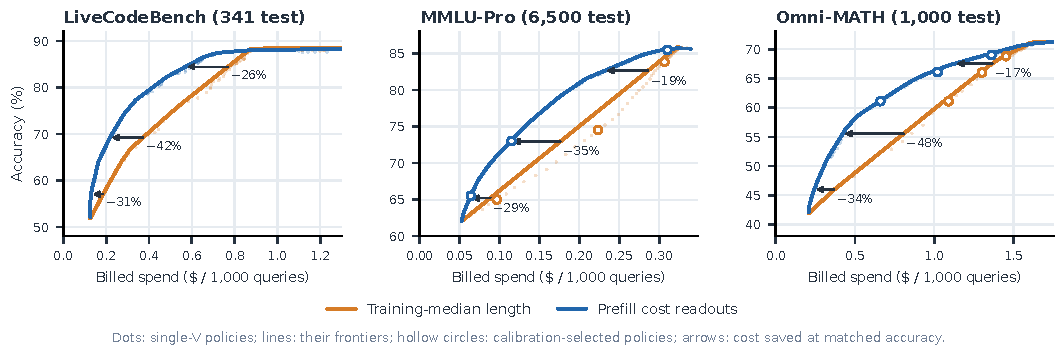
\includegraphics[width=\textwidth]{figures/shared_prefill_overview.pdf}
\caption{\textbf{Shared prefill and fresh routing curves.} (a) One frozen encoder supplies per-route success and cost readouts. (b) Fresh accuracy versus recorded spending for deterministic policies over the fixed $V$ grid. Lines connect observed operating points; they do not require randomized routing. Circles mark learned-cost policies selected on original calibration. \Cref{tab:fresh} reports cost and accuracy differences with pointwise intervals. Encoder overhead is excluded.}
\label{fig:overview}
\end{figure*}

\section{Cost Prediction and Routing}
For query $x$ and route $m$, let $p_m(x)$ be the probability of correctness and $c_m(x)$ the expected generation cost. A route is a model with a fixed reasoning-effort setting. We select one route before generation:
\begin{equation}
m^*(x;V)=\arg\max_m\{V\hat p_m(x)-\hat c_m(x)\},
\label{eq:route}
\end{equation}
where $V$ sets the value of a correct answer. A larger $V$ favors predicted correctness; a smaller $V$ gives cost more influence. Accuracy changes through the selected route, not abstention: every query receives an answer. There is no verifier or fallback call.

\paragraph{Features and prediction heads.}
We concatenate mean and last-token activations from eight Qwen3-4B layers, standardized on training data. Instruct-2507 is used on LiveCodeBench and MMLU-Pro; Thinking-2507 on Omni. Both readouts are regularized linear models. Logistic success heads fit a binomial likelihood over valid draws; penalty selection and Platt calibration use the first draw on calibration. Ridge cost heads fit log mean output length, selecting regularization by training-only cross-validation. Each route needs its own length labels.

\paragraph{Generation cost estimation.}
We exponentiate predicted log length, apply training-residual smearing, and match the route's training mean. For predicted output tokens $\hat\ell_m(x)$, input tokens $n_m^{\rm in}(x)$, and input/output rates in dollars per million,
\begin{equation}
\hat c_m(x)=\frac{r_m^{\rm in}n_m^{\rm in}(x)+r_m^{\rm out}\hat\ell_m(x)}{10^6}.
\label{eq:cost}
\end{equation}
The constant references substitute median valid training output length or mean problem--route training length. The empirical oracle substitutes observed problem--route mean length. Only the oracle uses evaluation lengths when selecting a route; all arms pay observed tokens after decisions are fixed.

\section{Experimental Protocol}
The main pools contain 892 LiveCodeBench problems~\cite{lcb}, all 500 Omni-MATH-500 problems from Omni-MATH~\cite{omni}, and a subject-stratified 1,000-question MMLU-Pro subset~\cite{mmlupro}. Train/calibration/test counts are 441/110/341, 275/75/150, and 550/150/300. The five routes are gpt-oss-20b at low/medium effort, deepseek-v4-flash, and gpt-oss-120b at medium/high effort. Approximately 16/12/8/6/3 valid draws per route are retained on LiveCodeBench and 4/3/3/2/2 on the other pools. Correctness and cost are estimated from all valid draws; generations are not treated as independent test problems.

\paragraph{Pricing and controls.}
We hold the recorded market rates fixed across arms: input/output dollars per million are 0.018/0.09 for gpt-oss-20b, 0.04704/0.09408 for deepseek-v4-flash, and 0.15/0.60 for gpt-oss-120b. Reported savings isolate target generation spend. The encoder pass is common to success-only and success-plus-cost routing, so these are incremental savings for an existing prefill router. Training and calibration exclude test problems.

\paragraph{Matched-accuracy evaluation.}
Each $V$ gives a deterministic policy and an observed accuracy--cost point. Fresh plots show these points directly. For the original descriptive frontiers, we also consider randomly sampling one of two policies per query. This gives their weighted mean accuracy and cost; the lower convex envelope contains the cheapest combinations. Mixture weights on those frontiers use evaluation outcomes. Let $C_{\rm arm}(a)$ denote frontier cost at accuracy $a$. Savings against median pricing are
\begin{equation}
G=1-\exp\!\left[\frac{1}{12}\sum_{j=1}^{12}
\log\frac{C_{\rm arm}(a_j)}{C_{\rm median}(a_j)}\right],
\label{eq:gain}
\end{equation}
using 12 targets over the interior 5--95\% of the band shared by the estimator, median reference, and oracle. Estimator bands can differ; differences in $G$ compare these summaries rather than direct savings at identical accuracies. Oracle $G$ measures headroom. We use 500 paired problem bootstrap resamples, retaining each problem's routes and draws together. These outcome-selected frontiers are descriptive. CARROT and ZeroRouter contrasts use 1,000 resamples; CARROT pairs share one accuracy band.

\paragraph{Fresh calibration-selected policies.}
We collect one generation per route on 6,500 disjoint MMLU-Pro and 1,000 disjoint Omni-MATH problems. Fitting and selection use original training/calibration data. Full solving prompts, including answer choices, match original encoder inputs. For each arm and historical target in $\{.60,.65,.70,.75,.80,.85\}$, we select the cheapest single-$V$ policy reaching at least the target accuracy on original calibration. We freeze it for fresh evaluation and report all reachable targets. No abstention or routing randomization is used. Fresh accuracy need not equal the calibration target. For savings $1-\bar C_{\rm learned}/\bar C_{\rm reference}$ and accuracy differences, 2,000 paired bootstraps resample problems within subject/difficulty strata, retaining planned weights. Percentile intervals are pointwise and conditional on fitted heads and policies, without multiplicity adjustment. An accuracy interval crossing zero does not establish equivalence. Calibration-selected two-policy mixtures are a supplementary sensitivity analysis.

\begin{table*}[t]
\centering
\footnotesize
\setlength{\tabcolsep}{3pt}
\begin{tabular}{lrrrrrr}
\toprule
Fresh set & \shortstack{Cal. target\\\%} & \shortstack{Fresh acc.\\ours, \%} & \shortstack{$\Delta$ acc. vs median\\pp [95\% CI]} & \shortstack{Savings vs median\\\% [95\% CI]} & \shortstack{$\Delta$ acc. vs mean\\pp [95\% CI]} & \shortstack{Savings vs mean\\\% [95\% CI]} \\
\midrule
MMLU-Pro & 60 & 61.90 & $+0.00 [+0.00, +0.00]$ & $0.0 [0.0, 0.0]$ & $+0.00 [+0.00, +0.00]$ & $0.0 [0.0, 0.0]$ \\
MMLU-Pro & 65 & 64.23 & $-0.33 [-0.97, +0.31]$ & $28.8 [22.5, 34.7]$ & $-0.76 [-1.41, -0.16]$ & $27.0 [23.6, 30.6]$ \\
MMLU-Pro & 70 & 66.80 & $-1.67 [-2.51, -0.88]$ & $47.2 [42.5, 51.3]$ & $-0.33 [-1.08, +0.45]$ & $33.9 [29.3, 38.4]$ \\
MMLU-Pro & 75 & 73.45 & $+1.29 [+0.35, +2.25]$ & $31.1 [25.6, 36.3]$ & $+1.66 [+0.81, +2.54]$ & $31.2 [25.7, 36.4]$ \\
MMLU-Pro & 80 & 76.93 & $-1.28 [-2.11, -0.42]$ & $29.3 [24.9, 33.5]$ & $-1.99 [-2.77, -1.25]$ & $32.7 [28.8, 36.4]$ \\
MMLU-Pro & 85 & 84.47 & $+0.33 [-0.01, +0.68]$ & $-5.1 [-7.0, -3.3]$ & $+3.17 [+2.61, +3.73]$ & $-15.3 [-17.6, -12.9]$ \\
\midrule
Omni-MATH & 60 & 56.40 & $+0.90 [-1.20, +2.90]$ & $29.4 [22.0, 36.4]$ & $+0.40 [-1.70, +2.40]$ & $34.3 [27.4, 40.4]$ \\
Omni-MATH & 65 & 58.70 & $+0.10 [-1.70, +2.00]$ & $24.9 [17.3, 31.6]$ & $+0.00 [-1.90, +1.90]$ & $29.2 [22.6, 35.4]$ \\
Omni-MATH & 70 & 62.90 & $-0.70 [-2.20, +0.80]$ & $16.0 [11.2, 20.9]$ & $-1.80 [-3.30, -0.30]$ & $19.6 [14.8, 24.4]$ \\
Omni-MATH & 75 & 68.10 & $-0.10 [-0.90, +0.70]$ & $3.3 [0.8, 6.0]$ & $+1.80 [+0.70, +2.90]$ & $-5.3 [-8.6, -2.1]$ \\
\bottomrule
\end{tabular}
\caption{\textbf{Fresh deterministic policies.} MMLU-Pro has 6,500 new problems and Omni-MATH has 1,000. For each target, each arm selects the cheapest single-$V$ policy reaching at least that accuracy on original calibration. Every query receives one answer; no routing randomization or abstention is used. Fresh accuracy need not equal the target or reference accuracy. Positive accuracy differences and savings favor learned costs. All reachable targets are shown. Intervals are pointwise paired stratified percentile bootstraps (2,000 resamples), conditional on the fitted heads and calibrated policies. Generation spending excludes encoder overhead.}
\label{tab:fresh}
\end{table*}


\begin{table*}[t]
\centering
\footnotesize
\setlength{\tabcolsep}{5pt}
\begin{tabular}{lrrr}
\toprule
Cost estimator & LiveCodeBench & Omni-MATH-500 & MMLU-Pro \\
\midrule
Embedding ensemble (MixLLM-style) & 14.1 [5.3, 21.0] & 12.5 [$-$2.4, 25.6] & 4.0 [$-$4.7, 14.9] \\
Prompt-feature GBM & 12.3 [0.7, 21.4] & 6.6 [$-$12.2, 21.2] & 9.8 [$-$4.5, 25.9] \\
Cost from success predictions & 34.1 [24.7, 40.9] & 21.0 [6.6, 33.7] & 9.2 [$-$2.2, 24.6] \\
Shared-prefill cost readouts (ours) & 35.6 [27.1, 41.9] & 21.9 [8.9, 33.5] & 30.7 [16.3, 43.2] \\
\bottomrule
\end{tabular}
\caption{\textbf{Original-test frontier summaries.} Savings $G$ (\%) against median-length pricing, with pointwise 95\% paired-problem bootstrap intervals. Each estimator has its own band; these are not direct savings against another learned estimator. Embedding and prompt-feature baselines are adaptations.}
\label{tab:main}
\end{table*}

\section{Results}
\paragraph{Fresh policy comparisons.}
\Cref{tab:fresh} reports both outcomes against both constants. At MMLU-Pro's 75\% calibration target, median-reference savings are 31.1\% [25.6, 36.3] with $+1.29$ [$+0.35$, $+2.25$] accuracy points. At Omni's 65\% target, savings are 24.9\% [17.3, 31.6], but accuracy is uncertain: $+0.10$ [$-1.70$, $+2.00$] points. MMLU-Pro's 70\% and 80\% targets lose accuracy against median pricing; its 85\% target spends more. Omni's 70\% target loses accuracy against mean pricing. The curves show where tradeoffs differ; we make no uniform or accuracy-equivalence claim.

\paragraph{Cost-estimator comparison.}
Original-test frontier savings are 35.6\% on LiveCodeBench, 21.9\% on Omni, and 30.7\% on MMLU-Pro (\cref{tab:main}), versus oracle savings of 46.0\%, 44.2\%, and 65.1\%.

The embedding baseline averages MLP, random-forest, and nearest-neighbor regressors on jina-code embeddings, adapting MixLLM's predictor family. The GBM uses prompt length, numbers, examples, constraints, and keywords. Both fit training log lengths. On MMLU-Pro, paired differences in $G$ are 26.7 points [12.4, 40.2] and 20.9 [3.8, 33.3]; on Omni they are inconclusive: 9.4 [$-4.4$, 24.2] and 15.2 [$-1.4$, 34.1]. These compare summaries over potentially different bands, not direct spending ratios at identical accuracy. Encoder size and regression design also differ.

\paragraph{Costs inferred from success predictions.}
We regress log length on predicted success logits and their squares, holding success predictions fixed in routing. This control saves 34.1\% on LiveCodeBench and 21.0\% on Omni; differences in $G$ from dedicated readouts are inconclusive. On MMLU-Pro it saves 9.2\%, versus 30.7\%: a paired summary difference of 21.5 points [8.5, 30.3].

On MMLU-Pro, adding subject labels to success-derived pricing raises $G$ to 22.3\%, accounting for roughly 60\% of the summary difference. Subject variation may partly explain the cost signal; this does not isolate variation in reasoning requirements.

\paragraph{CARROT and ZeroRouter comparisons.}
On original test sets, we evaluate CARROT's MiniLM encoder with cosine kNN cost prediction, holding our success scores fixed. Direct savings over a shared pairwise frontier band are 33.6\% [26.4, 40.3] on LiveCodeBench, 14.0\% [1.7, 24.2] on Omni, and 14.4\% [$-0.3$, 26.6] on MMLU-Pro. The full-router comparison gives 20.2\% [11.0, 26.9], 19.9\% [6.3, 32.3], and 5.2\% [$-12.5$, 20.5]. This comparison excludes CARROT's RoBERTa and OpenAI-embedding variants.

Our calibration-selected ZeroRouter reimplementation uses MAP item-response estimates, difficulty-bin pricing, and 4B features. Differences in original-test savings summaries are $+17.5$ [9.8, 24.9] points on LiveCodeBench, with inconclusive differences on MMLU-Pro ($+9.3$ [$-2.6$, 21.5]) and Omni ($+2.8$ [$-10.7$, 16.6]). Neither comparison includes expansion problems.

\paragraph{Results on additional datasets.}
CodeContests~\cite{codecontests}, TACO~\cite{taco}, and BigCodeBench~\cite{bigcodebench} have oracle savings of 21.8\%, 36.1\%, and 20.2\%, yet learned gains of 2.0\%, 2.1\%, and $-3.3\%$ have intervals spanning zero. RouterBench~\cite{routerbench} has 10.5\% headroom. Different models, prices, and accuracy ladders prevent attributing these differences to reasoning alone; supplementary controls give further detail.

\section{Discussion and Limitations}
Each route needs training output-length labels; the pools cover five configurations from two model families. MixLLM and ZeroRouter are adaptations; CARROT scope is limited to MiniLM/kNN. Pointwise intervals omit training and calibration-selection uncertainty and do not support selecting the strongest target after evaluation. Bootstrap inference assumes independent problems within strata. Fresh results use recorded generations and planned reference-stratum weights. The pipeline was corrected after outcomes were observed, and the deterministic follow-up was specified after the mixture results were examined; neither is newly preregistered. Encoder overhead is excluded. Broader model families and fresh comparisons with learned baselines remain needed.

\section{Conclusion}
Shared prefill activations support cost estimates for several reasoning routes. On new MMLU-Pro and Omni-MATH problems, calibration-selected policies reduce spending at several operating points, with accuracy differences reported separately. The result varies with the target and reference estimator; comparisons with other learned predictors remain mixed. Separate cost prediction can improve routing, but the evidence does not establish a uniform advantage.

\balance
{\small
\bibliographystyle{ieee_fullname}
\bibliography{references}
}
\end{document}
